\section{Beispielkrams}
Beispielabschnitt, in den ich die am meisten benutzen Auszeichnungen nutze:

\emph{Betonung, kursiv}

\begin{figure}[ht!]
    \centering
    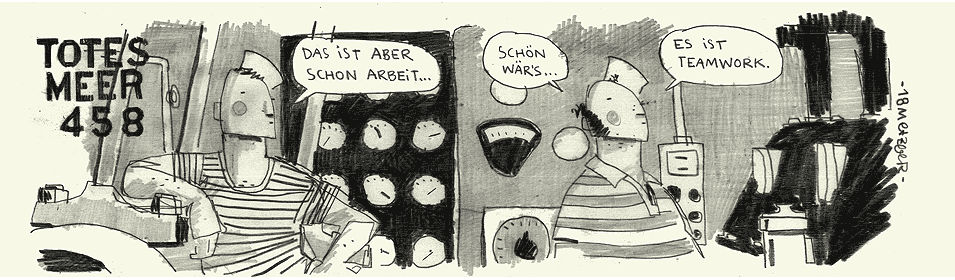
\includegraphics[width=\textwidth]{pics/test.png}
    \caption{Eine Beispielunterschrift unter einem Beispielbild}
    \label{fig:test}
\end{figure}

Benötigte Pakete:
\begin{itemize}

  \item texlive-bibtexextra
  \item texlive-core
  \item texlive-latexextra
  \item texlive-science
  \item Alle Pakete gibt es auch für Debian
  \item (für eine nummerierte Liste nutzt man \emph{enumerate} anstelle von
    \emph{itemize})

\end{itemize}

Technische Begriffe\footnote{Das ist eine Fußnote} oder Code im Fließtext:
\texttt{com.github.sgelb.arcs}

Auf das Label aus der Abbildung kann man sich beziehen, die Nummerierung
geschieht automatisch: siehe Abbildung~\ref{fig:test}).


\textbf{Codeblock:}

\begin{lstlisting}
connect(ui->nextBtn, &QPushButton::clicked, this,
        &MainWindow::nextTrack);
\end{lstlisting}

Am Ende noch eine URL, die sich natürlich im pdf Anklicken lässt:
\url{http://qt-project.org/doc/qt-5/qmediaplayer.html}

Mein workflow sieht in der Regel so aus, dass ich aus vim heraus das pdf
erstelle:

\texttt{:!pdflatex \%}\footnote{das Ausrufezeichen ruft einen
externen Befehl auf, das Prozentzeichen steht für das gesamte Dokument}

Einmal erstellt, öffne ich das pdf und da die meisten pdf-Viewer Änderungen
erkennen, wird das angezeigte pdf bei jeder Neugenerierung aktualisiert.
Manchmal sind zwei oder drei Aufrufe von \texttt{pdflatex} nötig, um
Inhaltsverzeichnis etc korrekt zu erstellen.

Quellenangaben sind in \texttt{references.bib} im BibText-Format
\citep{wiki:bibtex} gelistet und können mit dem entsprechen Befehl eingefügt
werden. Das ist ein absolutes Killerfeature von Tex, aber werden wir nicht
brauchen, darum gehe ich da nicht weiter drauf ein. Geiler Scheiß:
\url{http://www.rtwilson.com/academic/autozotbib},
\url{http://manas.tungare.name/software/isbn-to-bibtex/} und
\url{http://lead.to/amazon/en/?key=OpenCV&si=owb&op=bt&bn=&so=ta&ht=de}




